\subsection{Model \textit{Use case}}
\label{subsec:model-usecase}
Dari beberapa kebutuhan fungsional serta karakteristik pengguna, dapat dibuat \textit{use case} yang mengelompokan serta menggambarkan relasi antara aktor dan aksi yang dapat dilakukan. Use case akan memiliki identifikasi yang berawalan dengan UC diikuti oleh dua angka. Use case dapat dilihat secara detail pada tabel \ref{tab:penjelasan-usecase-diagram}

Dari pemetaan \textit{Use case} pada tabel \ref{tab:penjelasan-usecase-diagram}, dapat dibuat sebuah diagram yang menghubungkan relasi antara aktor dengan usecasenya. Relasi  aktor dengan kapabilitas fungsional sistem dapat dilihat pada diagram use case berikut.

\begin{figure}[ht]
  \centering
  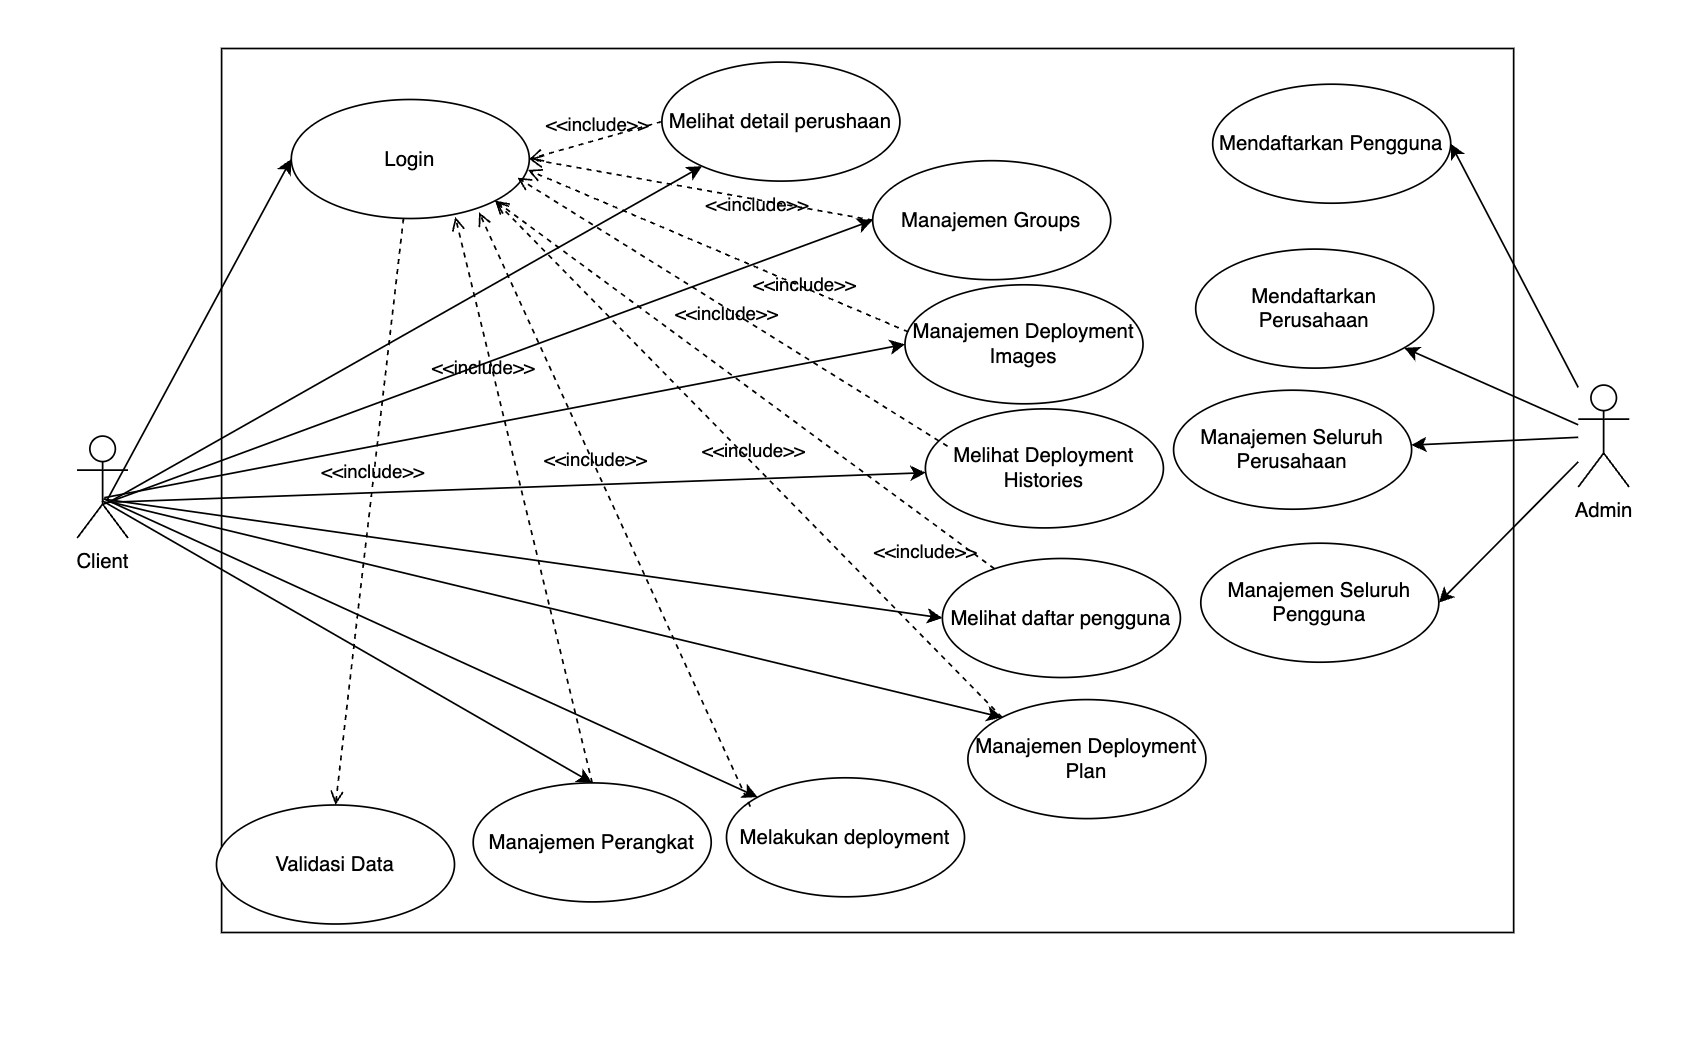
\includegraphics[width=1\textwidth]{resources/chapter-3/usecase-diagram.jpg}
  \caption{Usecase Diagram}
  \label{fig:usecase-diagram}
\end{figure}